The PRT Model calculates three-dimensional, advective particle trajectories in flowing groundwater. The PRT Model is designed to work with the Groundwater Flow (GWF) Model \citep{modflow6gwf} and uses the same spatial discretization, which may be represented using either a structured (DIS) or an unstructured (DISV) grid. The PRT Model replicates much of the functionality of MODPATH 7 \citep{pollock2016modpath7} and offers support for a much broader class of unstructured grids. The PRT Model can be run in the same simulation as the associated GWF Model or in a separate simulation that reads previously calculated flows from a binary budget file. The version of the PRT Model documented here does not support grids of DISU type, tracking of particles through advanced stress package features such as lakes or streams reaches, or exchange of particles between PRT models.

This section describes the data files for a \mf Particle Tracking (PRT) Model.  A PRT Model is added to the simulation by including a PRT entry in the MODELS block of the simulation name file.  There are currently two types of spatial discretization approaches that can be used with the PRT Model: DIS and DISV.  The input instructions for these three packages are not described here in this section on PRT Model input; input instructions for these three packages are described in the section on GWF Model input.  Note that for a PRT Model, the maximum number of vertices for a cell in a DISV grid is limited to 8.

The PRT Model is designed to permit input to be gathered, as it is needed, from many different files.  Likewise, results from the model calculations can be written to a number of output files. Details about the files used by each package are provided in this section on the PRT Model Instructions.

The PRT Model reads a file called the Name File, which specifies most of the files that will be used in a simulation. Several files are always required whereas other files are optional depending on the simulation. The Output Control Package receives instructions from the user to control the amount and frequency of output.  Details about the Name File and the Output Control Package are described in this section.

For the PRT Model, ``flows'' (unless stated otherwise) represent particle mass ``flow'' in mass per time, rather than groundwater flow.  Each particle is currently assigned unit mass, and the numerical value of the flow can be interpreted as particles per time.

\subsection{Units of Length and Time}
The PRT Model formulates the particle trajectory equations without using prescribed length and time units. Any consistent units of length and time can be used when specifying the input data for a simulation. This capability gives a certain amount of freedom to the user, but care must be exercised to avoid mixing units.  The program cannot detect the use of inconsistent units.

\subsection{Time Stepping}
In \mf time step lengths are controlled by the user and specified in the Temporal Discretization (TDIS) input file.  When the flow model and particle-tracking model run in the same simulation, the time step length specified in TDIS is used for both models.  If the PRT Model runs in a separate simulation, the time discretization may differ.  Instructions for specifying time steps are described in the TDIS section of this user guide; additional information on GWF and PRT configurations are in the Flow Model Interface section.  By default, the PRT model will terminate particles at the end of the simulation's final time step; PRT can be configured to extend tracking until particles terminate naturally (i.e. at boundary conditions, sinks, or specified stop times) via Particle Release Point (PRP) package settings.

\subsection{Specifying Cell Face Flows using IFLOWFACE}

By default, flows associated with stress packages are assumed to be distributed uniformly over the volume of a cell. Distributed external inflows and outflows are reflected in the cell-cell flows calculated by the GWF Model, but they are not directly involved in determining the normal face velocities used to track a particle through the cell. The user can optionally assign a flow associated with a stress package to any face of the cell. Assignment of external flows is done by setting the value of an auxiliary package variable called IFLOWFACE to a value that corresponds to one of the cell faces. To accommodate non-rectangular cells, the IFLOWFACE numbering scheme in the PRT Model is based on clockwise ordering of the lateral cell faces. For a DIS-grid cell, IFLOWFACE = 1 corresponds to the ``western'' face, i.e., the face parallel to the y axis that has the lesser x coordinate. For a DISV-grid cell, IFLOWFACE = 1 corresponds to the face that extends in the clockwise direction from the first vertex listed for that cell in the CELL2D input block. IFLOWFACE numbering of lateral cell faces proceeds in clockwise direction. IFLOWFACE = -2 corresponds to the cell bottom, and IFLOWFACE = -1 corresponds to the cell top.

\subsection{Particle Mass Budget}
A summary of all inflow (sources) and outflow (sinks) of particle mass is called a mass budget.  The particle mass budget is printed to the PRT Model Listing File for selected time steps.  In the current implementation, each particle is assigned unit mass, and the numerical value of the flow can be interpreted as particles per time.

\subsection{Particle Release and Tracking in Inactive, Dry-But-Active, and Partially Saturated Cells}

The motion of a particle is determined by the groundwater velocity field in which the particle is immersed. In a fully saturated cell, or the saturated portion of a partially saturated cell, the velocity field is calculated from the flows entering and exiting the cell. In a completely dry cell, or the dry portion of a partially saturated cell, the fate of a particle depends on whether the cell is an active part of the flow simulation, whether the particle is in a dry or wet part of the cell, and user-selected options.

A cell can be inactive either because it has been removed from the active simulation using the IDOMAIN array or because it is completely dry, i.e., the head in the cell is below the bottom elevation of the cell. Deactivation of completely dry cells is the default behavior in MODFLOW 6. However, when the Newton-Raphson formulation is used to solve for groundwater flow, completely dry cells remain active. Particle tracking through inactive and dry-but-active cells is discussed in detail below.

Release-time and tracking-time considerations are described (and implemented) separately.

\subsubsection{Release}

At release time, PRT decides whether to release each particle or terminate it unreleased.

If the cell into which the particle is being released is inactive, behavior is determined by the DRAPE option. If the DRAPE option is enabled, the particle will be released from the top-most active cell beneath it, if any. If there is no active cell underneath the particle in any layer, or if DRAPE is not enabled, the particle will terminate unreleased (with status code 8).

If the cell into which the particle is being released is active, the particle will be released at the user-specified location, even if that location is in the dry portion of the cell or the cell is dry-but-active.

Note that for a dry-but-active cell the DRAPE option has no effect. In that case, the particle is released into the cell, and its subsequent behavior can be configured using the DRY\_TRACKING\_METHOD option discussed below.

\subsubsection{Tracking}

During tracking, the fate of a particle depends on the status of the cell that contains the particle, whether the particle is in a wet or dry part of the cell, and the DRY\_TRACKING\_METHOD option.

A particle immersed in the groundwater flow field during a given time step can end up in an inactive cell, a dry-but-active cell, or the dry part of a partially saturated cell if the water table drops on the next time step.

A particle that finds itself in an inactive cell will terminate with status code 7. This is consistent with the behavior of MODPATH 7.

Dry-but-active cells can occur when the Newton-Raphson formulation is used to solve for groundwater flow. As discussed above, particles can be released into dry-but-active cells.

A particle in a dry-but-active cell, or above the water table in a partially saturated cell, which we call a dry particle, need not terminate. The PRP package provides a DRY\_TRACKING\_METHOD option that determines how dry particles should behave. Supported values are DROP (the default), STOP, and STAY.

If DROP is selected, or if a DRY\_TRACKING\_METHOD is unspecified, a dry particle is passed vertically and instantaneously to the water table (if the cell is partially saturated) or to the bottom of the cell (if the cell is dry). This repeats (i.e., the particle may drop through multiple cells) until it reaches the water table. Tracking then proceeds as usual. If the vertical column containing the particle is entirely dry, the particle will terminate upon reaching the bottom
of the model grid.

If STOP is selected, dry particles will be terminated.

If STAY is selected, a dry particle will remain stationary until a) the water table rises and tracking can continue, b) the particle terminates due to reaching its STOPTIME or STOPTRAVELTIME, or c) the simulation ends.

\subsection{Particle Track Output}

The PRT Model supports both binary and CSV particle track output files. A particle track CSV file contains the output data in tabular format. The first line of the CSV file contains column names. Each subsequent line in the file contains a row of data for a single particle track record, with the following fields:

\vspace{5mm}
\noindent Column 0: \texttt{`KPER'} {\color{red} \footnotesize{INTEGER}} \\
\noindent Column 1: \texttt{`KSTP'} {\color{red} \footnotesize{INTEGER}} \\
\noindent Column 2: \texttt{`IMDL'} {\color{red} \footnotesize{INTEGER}} \\
\noindent Column 3: \texttt{`IPRP'} {\color{red} \footnotesize{INTEGER}} \\
\noindent Column 4: \texttt{`IRPT'} {\color{red} \footnotesize{INTEGER}} \\
\noindent Column 5: \texttt{`ILAY'} {\color{red} \footnotesize{INTEGER}} \\
\noindent Column 6: \texttt{`ICELL'} {\color{red} \footnotesize{INTEGER}} \\
\noindent Column 7: \texttt{`IZONE'} {\color{red} \footnotesize{INTEGER}} \\
\noindent Column 8: \texttt{`ISTATUS'} {\color{red} \footnotesize{INTEGER}} \\
\noindent Column 9: \texttt{`IREASON'} {\color{red} \footnotesize{INTEGER}} \\
\noindent Column 10: \texttt{`TRELEASE'} {\color{red} \footnotesize{DOUBLE}} \\
\noindent Column 11: \texttt{`T'} {\color{red} \footnotesize{DOUBLE}} \\
\noindent Column 12: \texttt{`X'} {\color{red} \footnotesize{DOUBLE}} \\
\noindent Column 13: \texttt{`Y'} {\color{red} \footnotesize{DOUBLE}} \\
\noindent Column 14: \texttt{`Z'} {\color{red} \footnotesize{DOUBLE}} \\
\noindent Column 15: \texttt{`NAME'} {\color{red} \footnotesize{CHARACTER(LEN=LENBOUNDNAME)}} \\

\vspace{2mm}
\noindent where

\begin{description} \itemsep0pt \parskip0pt \parsep0pt
\item \texttt{KPER} is the stress period number
\item \texttt{KSTP} is the time step number
\item \texttt{IMDL} is the number of the model the particle originated in
\item \texttt{IPRP} is the number of the particle release point (PRP) package the particle originated in
\item \texttt{IRPT} is the release point number
\item \texttt{ILAY} is the layer number
\item \texttt{ICELL} is the cell number
\item \texttt{IZONE} is the zone number
\item \texttt{ISTATUS} is the particle status code
\item \texttt{IREASON} is the reporting reason code
\item \texttt{TRELEASE} is the particle release time
\item \texttt{T} is the particle tracking time
\item \texttt{X} is the particle x coordinate
\item \texttt{Y} is the particle y coordinate
\item \texttt{Z} is the particle z coordinate
\item \texttt{NAME} is the name of the particle release point
\end{description}

The ISTATUS field indicates the status of the particle:

\begin{description} \itemsep0pt \parskip0pt \parsep0pt
\item \texttt{0}: particle was released
\item \texttt{1}: particle is being actively tracked
\item \texttt{2}: particle terminated at a boundary face
\item \texttt{3}: particle terminated in a weak sink cell
\item \texttt{4}: \textit{unused}
\item \texttt{5}: particle terminated in a cell with no exit face
\item \texttt{6}: particle terminated in a stop zone
\item \texttt{7}: particle terminated in an inactive cell
\item \texttt{8}: particle terminated immediately upon release into a dry cell
\item \texttt{9}: particle terminated in a subcell with no exit face
\end{description}

The IREASON field indicates the reason the particle track record was saved:

\begin{description} \itemsep0pt \parskip0pt \parsep0pt
\item \texttt{0}: particle was released
\item \texttt{1}: particle exited a cell
\item \texttt{2}: time step ended
\item \texttt{3}: particle terminated
\item \texttt{4}: particle entered a weak sink cell
\item \texttt{5}: user-specified tracking time
\end{description}

By default, the PRT Model reports all particle events. The user can optionally select which events are reported, as explained in the Output Control (OC) subsection. Because multiple tracking events may coincide (e.g. exiting a cell and exiting a weak sink cell), particle track records may be duplicates except for the ISTATUS and/or IREASON codes.

The binary particle track file contains the same particle track data in a record-based binary format explained in the Particle Track File subsection of the Description of Binary Output Files section.



\newpage
\subsection{PRT Model Name File}
The CHF Model Name File specifies the options and packages that are active for a CHF model.  The Name File contains two blocks: OPTIONS  and PACKAGES. The lines in each block can be in any order.  Files listed in the PACKAGES block must exist when the program starts. 

Comment lines are indicated when the first character in a line is one of the valid comment characters.  Commented lines can be located anywhere in the file. Any text characters can follow the comment character. Comment lines have no effect on the simulation; their purpose is to allow users to provide documentation about a particular simulation. 

\vspace{5mm}
\subsubsection{Structure of Blocks}
\lstinputlisting[style=blockdefinition]{./mf6ivar/tex/chf-nam-options.dat}
\lstinputlisting[style=blockdefinition]{./mf6ivar/tex/chf-nam-packages.dat}

\vspace{5mm}
\subsubsection{Explanation of Variables}
\begin{description}
\input{./mf6ivar/tex/chf-nam-desc.tex}
\end{description}

\begin{table}[H]
\caption{Ftype values described in this report.  The \texttt{Pname} column indicates whether or not a package name can be provided in the name file.  The capability to provide a package name also indicates that the CHF Model can have more than one package of that Ftype}
\small
\begin{center}
\begin{tabular*}{\columnwidth}{l l l}
\hline
\hline
Ftype & Input File Description & \texttt{Pname}\\
\hline
DISV1D6 & Discretization by Vertices in 1D Input File \\
DFW6 & Diffusive Wave Package \\ 
CXS6 & Cross Section Package \\ 
OC6 & Output Control Option \\
IC6 & Initial Conditions Package \\
STO6 & Storage Package \\
CHD6 & Constant Head Package & * \\ 
FLW6 & Inflow Package & * \\ 
PCP6 & Precipitation Package & * \\
EVP6 & Evaporation Package & * \\
ZDG6 & Zero-Depth Gradient Package & * \\ 
CDB6 & Critical Depth Boundary Package & * \\ 
OBS6 & Observations Option \\
\hline 
\end{tabular*}
\label{table:ftype-chf}
\end{center}
\normalsize
\end{table}

\vspace{5mm}
\subsubsection{Example Input File}
\lstinputlisting[style=inputfile]{./mf6ivar/examples/chf-nam-example.dat}



%\newpage
%\subsection{Structured Discretization (DIS) Input File}
%Discretization information for structured grids is read from the file that is specified by ``DIS6'' as the file type.  Only one discretization input file (DISU6, DISV6 or DIS6) can be specified for a model.

\vspace{5mm}
\subsubsection{Structure of Blocks}
\lstinputlisting[style=blockdefinition]{./mf6ivar/tex/gwf-dis-options.dat}
\lstinputlisting[style=blockdefinition]{./mf6ivar/tex/gwf-dis-dimensions.dat}
\lstinputlisting[style=blockdefinition]{./mf6ivar/tex/gwf-dis-griddata.dat}

\vspace{5mm}
\subsubsection{Explanation of Variables}
\begin{description}
\input{./mf6ivar/tex/gwf-dis-desc.tex}
\end{description}

\vspace{5mm}
\subsubsection{Example Input File}
\lstinputlisting[style=inputfile]{./mf6ivar/examples/gwf-dis-example.dat}


%\newpage
%\subsection{Discretization with Vertices (DISV) Input File}
%Discretization information for DISV grids is read from the file that is specified by ``DISV6'' as the file type.  Only one discretization input file (DISV6, DISU6 or DIS6) can be specified for a model.

The approach for numbering cell and cell vertices for the DISV Package is shown in figure~\ref{fig:gwf-fig3-2}.  The list of vertices for a cell must be in clockwise order.  Closing of the cell polygon by repeating the first vertex as the last vertex is not required in the present implementation.  Internally within the program, however, the first vertex number is added to the end of the vertex list in order to close the polygon.  Thus, users have the option for whether or not to close cell polygons.

\begin{figure}[ht]
	\centering
	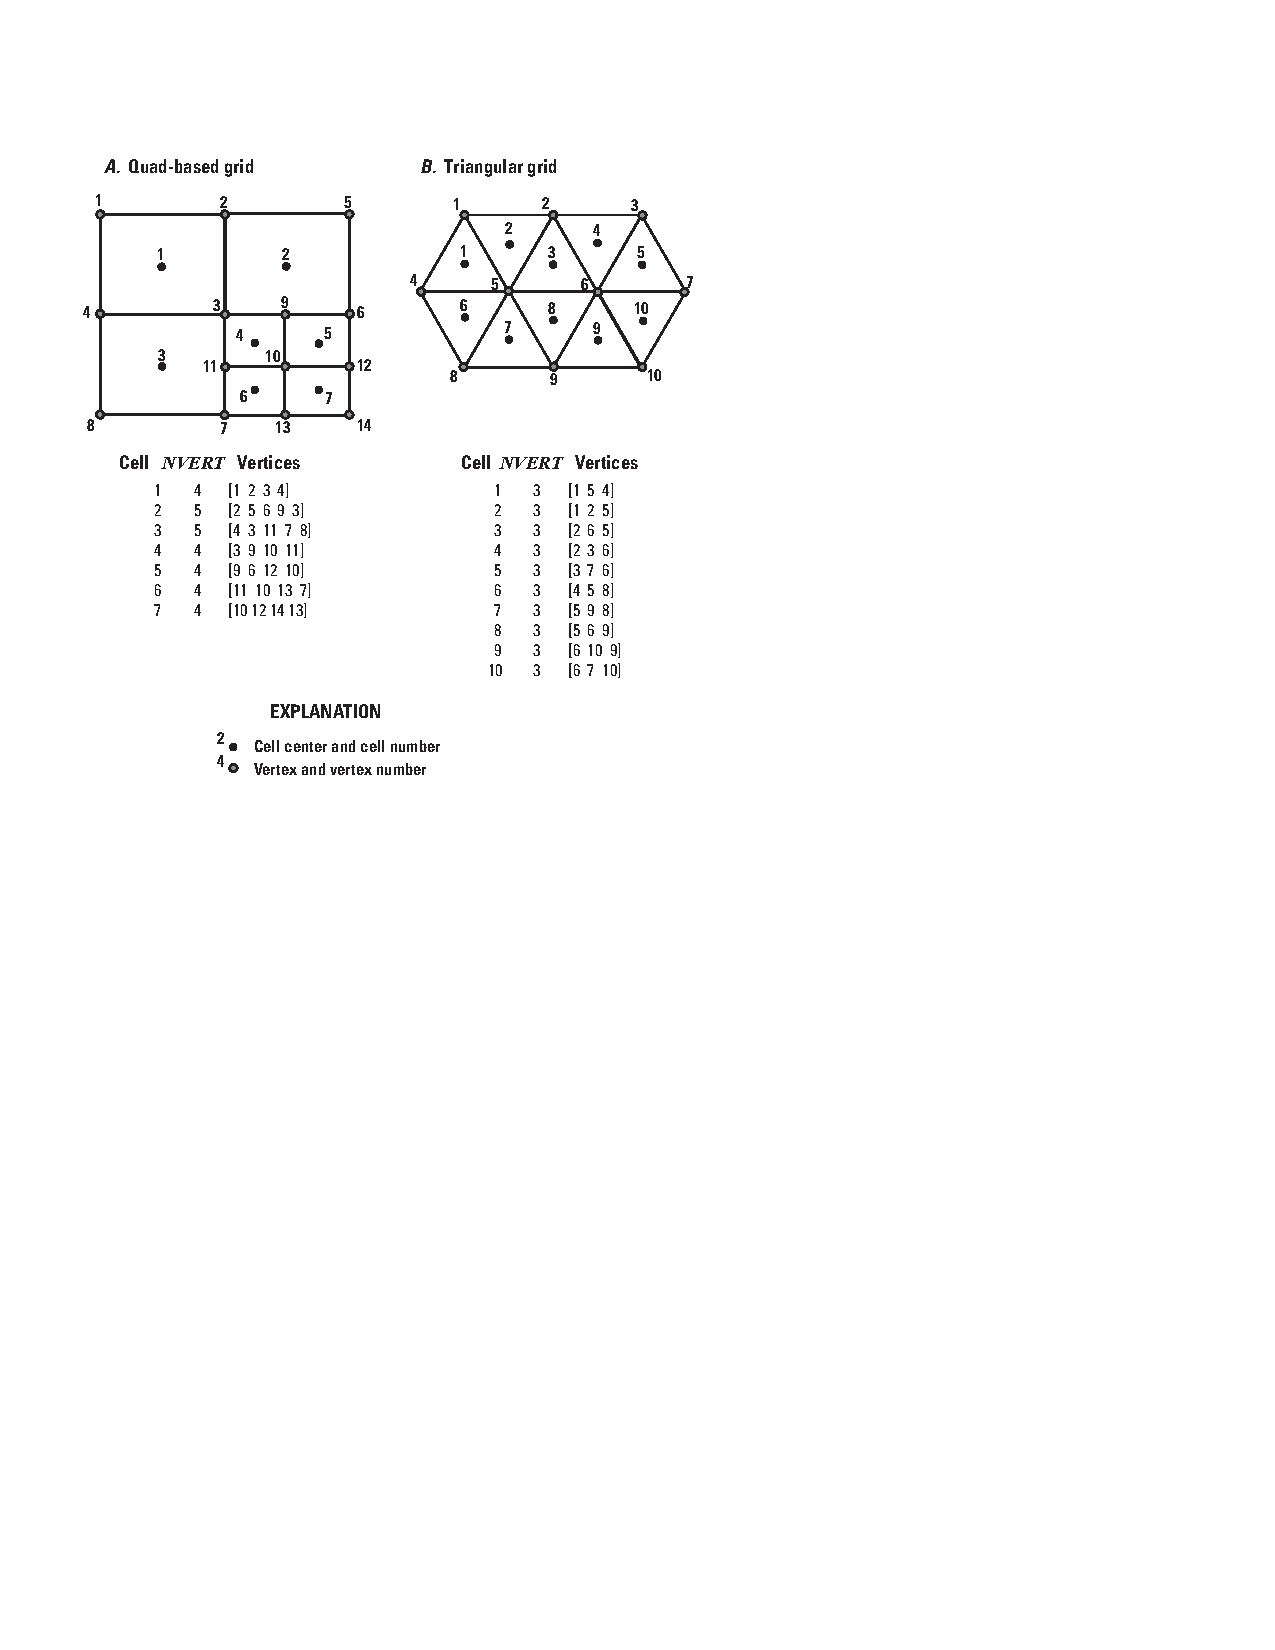
\includegraphics[scale=1.0]{Figures/gwf-fig3-2}
	\caption{Schematic diagram showing the vertices and cells defined using the Discretization by Vertices Package. The list of vertices used to define each cell must be in clockwise order.  From \cite{modflow6gwf}}
	\label{fig:gwf-fig3-2}
\end{figure}


\vspace{5mm}
\subsubsection{Structure of Blocks}
\lstinputlisting[style=blockdefinition]{./mf6ivar/tex/gwf-disv-options.dat}
\lstinputlisting[style=blockdefinition]{./mf6ivar/tex/gwf-disv-dimensions.dat}
\lstinputlisting[style=blockdefinition]{./mf6ivar/tex/gwf-disv-griddata.dat}
\lstinputlisting[style=blockdefinition]{./mf6ivar/tex/gwf-disv-vertices.dat}
\lstinputlisting[style=blockdefinition]{./mf6ivar/tex/gwf-disv-cell2d.dat}

\vspace{5mm}
\subsubsection{Explanation of Variables}
\begin{description}
\input{./mf6ivar/tex/gwf-disv-desc.tex}
\end{description}

\vspace{5mm}
\subsubsection{Example Input File}
\lstinputlisting[style=inputfile]{./mf6ivar/examples/gwf-disv-example.dat}


%\newpage
%\subsection{Unstructured Discretization (DISU) Input File}
%Discretization information for unstructured grids is read from the file that is specified by ``DISU6'' as the file type.  Only one discretization input file (DISU6, DISV6 or DIS6) can be specified for a model.

The shape and position of each cell can be defined using vertices.  This information is optional and is only read if the number of vertices (NVERT) in the DIMENSIONS block is specified and is assigned a value larger than zero.  If the vertices and two-dimensional cell information is provided in this file, then this information is also written to the binary grid file.  Providing this information may be useful for other postprocessing programs that read the binary grid file.

The DISU Package does not support the concept of layers, which is different from the DISU implementation in MODFLOW-USG.  In \mf~all grid input and output for models that use the DISU Package is entered or written as a one-dimensional array of size nodes.

The DISU VERTICES and CELL2D blocks are not required for all simulations.  These blocks are required if the XT3D or the SAVE\_SPECIFIC\_DISCHARGE options are specified in the NPF Package.  In general, it is recommended to include the VERTICES and CELL2D blocks. 

\vspace{5mm}
\subsubsection{Structure of Blocks}
\lstinputlisting[style=blockdefinition]{./mf6ivar/tex/gwf-disu-options.dat}
\lstinputlisting[style=blockdefinition]{./mf6ivar/tex/gwf-disu-dimensions.dat}
\lstinputlisting[style=blockdefinition]{./mf6ivar/tex/gwf-disu-griddata.dat}
\lstinputlisting[style=blockdefinition]{./mf6ivar/tex/gwf-disu-connectiondata.dat}
\lstinputlisting[style=blockdefinition]{./mf6ivar/tex/gwf-disu-vertices.dat}
\lstinputlisting[style=blockdefinition]{./mf6ivar/tex/gwf-disu-cell2d.dat}

\vspace{5mm}
\subsubsection{Explanation of Variables}
\begin{description}
\input{./mf6ivar/tex/gwf-disu-desc.tex}
\end{description}

\vspace{5mm}
\subsubsection{Example Input File}
\lstinputlisting[style=inputfile]{./mf6ivar/examples/gwf-disu-example.dat}



\newpage
\subsection{Model Input (MIP) Package}
Model Input (MIP) Package information is read from the file that is specified by ``MIP6'' as the file type.  The MIP Package is required, and only one MIP Package can be specified for a PRT model.  The information read by the MIP Package pertains to the entire PRT model.

\vspace{5mm}
\subsubsection{Structure of Blocks}
\lstinputlisting[style=blockdefinition]{./mf6ivar/tex/prt-mip-options.dat}
\lstinputlisting[style=blockdefinition]{./mf6ivar/tex/prt-mip-griddata.dat}

\vspace{5mm}
\subsubsection{Explanation of Variables}
\begin{description}
\input{./mf6ivar/tex/prt-mip-desc.tex}
\end{description}

\vspace{5mm}
\subsubsection{Example Input File}
\lstinputlisting[style=inputfile]{./mf6ivar/examples/prt-mip-example.dat}


\newpage
\subsection{Particle Release Point (PRP) Package}
Particle Release Point (PRP) Package information is read from the file that is specified by ``PRP6'' as the file type.  More than one PRP Package can be specified for a PRT model. 

The PRP Package offers multiple ways to specify particle release times.  Particle release times may either be provided explicitly, relative to the simulation start time, or configured relative to the time discretization of stress periods via period block settings.  When multiple ways of specifying release times are used together, the resulting set of release times is the union of the times specified by each method.

This package contains options to configure how particles behave in dry conditions. Each of these is described in detail below. Their interaction is summarized in the PRT chapter introduction.

\vspace{5mm}
\subsubsection{Structure of Blocks}
\lstinputlisting[style=blockdefinition]{./mf6ivar/tex/prt-prp-options.dat}
\lstinputlisting[style=blockdefinition]{./mf6ivar/tex/prt-prp-dimensions.dat}
\lstinputlisting[style=blockdefinition]{./mf6ivar/tex/prt-prp-packagedata.dat}
\lstinputlisting[style=blockdefinition]{./mf6ivar/tex/prt-prp-releasetimes.dat}
\vspace{5mm}
\noindent \textit{FOR ANY STRESS PERIOD}
\lstinputlisting[style=blockdefinition]{./mf6ivar/tex/prt-prp-period.dat}
\packageperioddescription \: If no PERIOD block is specified for any period, a single particle is released from each release point at the beginning of the simulation.
%\noindent All of the stress period information in a PERIOD block will apply only to that stress period; the information will not continue to apply for subsequent stress periods.  Note that this behavior is different from the simple stress packages (CHD, WEL, DRN, RIV,
%GHB, RCH and EVT) and the advanced stress packages (MAW, SFR, LAK, and UZF).

\vspace{5mm}
\subsubsection{Explanation of Variables}
\begin{description}
\input{./mf6ivar/tex/prt-prp-desc.tex}
\end{description}

\vspace{5mm}
\subsubsection{Example Input File}
\lstinputlisting[style=inputfile]{./mf6ivar/examples/prt-prp-example.dat}



\newpage
\subsection{Output Control (OC) Option}
Input to the Output Control Option of the Surface Water Flow Model is read from the file that is specified as type ``OC6'' in the Name File. If no ``OC6'' file is specified, default output control is used. The Output Control Option determines how and when outflows are printed to the listing file and/or written to a separate binary output file.  Under the default, outflow and overall flow budget are written to the Listing File at the end of every stress period. The default printout format for concentrations is 10G11.4.  The outflow and overall flow budget are also written to the list file if the simulation terminates prematurely due to failed convergence.

\vspace{5mm}
\subsubsection{Structure of Blocks}
\vspace{5mm}

\noindent \textit{FOR EACH SIMULATION}
\lstinputlisting[style=blockdefinition]{./mf6ivar/tex/olf-oc-options.dat}
\vspace{5mm}
\noindent \textit{FOR ANY STRESS PERIOD}
\lstinputlisting[style=blockdefinition]{./mf6ivar/tex/olf-oc-period.dat}

\vspace{5mm}
\subsubsection{Explanation of Variables}
\begin{description}
\input{./mf6ivar/tex/olf-oc-desc.tex}
\end{description}

\vspace{5mm}
\subsubsection{Example Input File}
\lstinputlisting[style=inputfile]{./mf6ivar/examples/olf-oc-example.dat}


\newpage
\subsection{Flow Model Interface (FMI) Package}
Flow Model Interface (FMI) Package information is read from the file that is specified by ``FMI6'' as the file type.  The FMI Package file is required only if the PRT Model is running in a separate simulation from a previously run GWF Model. If the PRT Model is coupled to a GWF Model by an exchange, the FMI Package file is not required. Only one FMI Package can be specified for a PRT model.

The PRT Model needs groundwater flows for model grid cells, for boundary conditions, and for other terms, such as the flow of water in or out of storage.  The FMI Package is the interface between the PRT Model and simulated groundwater flows provided by a corresponding GWF Model that is running concurrently within the simulation or from binary budget files that were created from a previous GWF model run.  The following are several different FMI simulation cases:

\begin{itemize}

\item Flows are provided by a corresponding GWF Model running in the same simulation---in this case, all groundwater flows are calculated by the corresponding GWF Model and provided through FMI to the transport model.  This is a common use case in which the user wants to run the flow and particle-tracking models as part of a single simulation.  The GWF and PRT models must be part of a GWF-PRT Exchange that is listed in mfsim.nam.  If a GWF-PRT Exchange is specified by the user, then the user does not need to specify an FMI Package input file for the simulation, unless an FMI option is needed.  If a GWF-PRT Exchange is specified and the FMI Package is specified, then the PACKAGEDATA block below is not read or used.

\item Flows are provided from a previous GWF model simulation---in this case FMI should be provided in the PRT name file and the head and budget files should be listed in the FMI PACKAGEDATA block.  In this case, FMI reads the simulated head and flows from these files and makes them available to the particle-tracking model.  There are some additional considerations when the heads and flows are provided from binary files.

\begin{itemize}
\item The binary budget file must contain the simulated flows for all of the packages that were included in the GWF model run.  Saving of flows can be activated for all packages by specifying ``SAVE\_FLOWS'' as an option in the GWF name file.  The GWF Output Control Package must also have ``SAVE BUDGET ALL'' specified.  The easiest way to ensure that all flows and heads are saved is to use the following simple form of a GWF Output Control file:

\begin{verbatim}
BEGIN OPTIONS
  HEAD FILEOUT mymodel.hds
  BUDGET FILEOUT mymodel.bud
END OPTIONS

BEGIN PERIOD 1
  SAVE HEAD ALL
  SAVE BUDGET ALL
END PERIOD
\end{verbatim}

\item The binary budget file must have the same number of budget terms listed for each time step.  This will always be the case when the binary budget file is created by \mf.
\item The binary heads file must have heads saved for all layers in the model.  This will always be the case when the binary head file is created by \mf.  This was not always the case as previous MODFLOW versions allowed different save options for each layer.
\item If the binary budget and head files have more than one time step for a single stress period, then the budget and head information must be contained within the binary file for every time step in the simulation stress period.
\item The binary budget and head files must correspond in terms of information stored for each time step and stress period.
\item If the binary budget and head files have information provided for only the first time step of a given stress period, this information will be used for all time steps in that stress period in the PRT simulation. If the final (or only) stress period in the binary budget and head files contains data for only one time step, this information will be used for any subsequent time steps and stress periods in the PRT simulation. This makes it possible to provide flows, for example, from a steady-state GWF stress period and have those flows used for all PRT time steps in that stress period, for all remaining time steps in the PRT simulation, or for all time steps throughout the entire PRT simulation. With this option, it is possible to have smaller time steps in the PRT simulation than the time steps used in the GWF simulation. Note that this cannot be done when the GWF and PRT models are run in the same simulation, because in that case, both models are solved over the same sequence of time steps and stress periods, as listed in the TDIS Package. The option to read flows from a previous GWF simulation via Flow Model Interface may offer an efficient alternative to running both models in the same simulation, but comes at the cost of having potentially very large budget files.
\item The binary grid file is optional but recommended, as it allows \mf to verify that the GWF and PRT model grids are identical.
\end{itemize}

\end{itemize}

\noindent Determination of which FMI use case to invoke requires careful consideration of the different advantages and disadvantages of each case.  For example, running PRT and GWF in the same simulation can often be faster because GWF flows are passed through memory to the PRT model instead of being written to files.  The disadvantage of this approach is that the same time step lengths must be used for both GWF and PRT.  Ultimately, it should be relatively straightforward to test different ways in which GWF and PRT interact and select the use case most appropriate for the particular problem. 

\vspace{5mm}
\subsubsection{Structure of Blocks}
\lstinputlisting[style=blockdefinition]{./mf6ivar/tex/prt-fmi-packagedata.dat}

\vspace{5mm}
\subsubsection{Explanation of Variables}
\begin{description}
\input{./mf6ivar/tex/prt-fmi-desc.tex}
\end{description}

\vspace{5mm}
\subsubsection{Example Input File}
\lstinputlisting[style=inputfile]{./mf6ivar/examples/prt-fmi-example.dat}


